% Options for packages loaded elsewhere
\PassOptionsToPackage{unicode}{hyperref}
\PassOptionsToPackage{hyphens}{url}
%
\documentclass[
  man, donotrepeattitle,mask,floatsintext]{apa7}
\usepackage{amsmath,amssymb}
\usepackage{lmodern}
\usepackage{iftex}
\ifPDFTeX
  \usepackage[T1]{fontenc}
  \usepackage[utf8]{inputenc}
  \usepackage{textcomp} % provide euro and other symbols
\else % if luatex or xetex
  \usepackage{unicode-math}
  \defaultfontfeatures{Scale=MatchLowercase}
  \defaultfontfeatures[\rmfamily]{Ligatures=TeX,Scale=1}
\fi
% Use upquote if available, for straight quotes in verbatim environments
\IfFileExists{upquote.sty}{\usepackage{upquote}}{}
\IfFileExists{microtype.sty}{% use microtype if available
  \usepackage[]{microtype}
  \UseMicrotypeSet[protrusion]{basicmath} % disable protrusion for tt fonts
}{}
\makeatletter
\@ifundefined{KOMAClassName}{% if non-KOMA class
  \IfFileExists{parskip.sty}{%
    \usepackage{parskip}
  }{% else
    \setlength{\parindent}{0pt}
    \setlength{\parskip}{6pt plus 2pt minus 1pt}}
}{% if KOMA class
  \KOMAoptions{parskip=half}}
\makeatother
\usepackage{xcolor}
\usepackage{graphicx}
\makeatletter
\def\maxwidth{\ifdim\Gin@nat@width>\linewidth\linewidth\else\Gin@nat@width\fi}
\def\maxheight{\ifdim\Gin@nat@height>\textheight\textheight\else\Gin@nat@height\fi}
\makeatother
% Scale images if necessary, so that they will not overflow the page
% margins by default, and it is still possible to overwrite the defaults
% using explicit options in \includegraphics[width, height, ...]{}
\setkeys{Gin}{width=\maxwidth,height=\maxheight,keepaspectratio}
% Set default figure placement to htbp
\makeatletter
\def\fps@figure{htbp}
\makeatother
\setlength{\emergencystretch}{3em} % prevent overfull lines
\providecommand{\tightlist}{%
  \setlength{\itemsep}{0pt}\setlength{\parskip}{0pt}}
\setcounter{secnumdepth}{-\maxdimen} % remove section numbering
% Make \paragraph and \subparagraph free-standing
\ifx\paragraph\undefined\else
  \let\oldparagraph\paragraph
  \renewcommand{\paragraph}[1]{\oldparagraph{#1}\mbox{}}
\fi
\ifx\subparagraph\undefined\else
  \let\oldsubparagraph\subparagraph
  \renewcommand{\subparagraph}[1]{\oldsubparagraph{#1}\mbox{}}
\fi
\newlength{\cslhangindent}
\setlength{\cslhangindent}{1.5em}
\newlength{\csllabelwidth}
\setlength{\csllabelwidth}{3em}
\newlength{\cslentryspacingunit} % times entry-spacing
\setlength{\cslentryspacingunit}{\parskip}
\newenvironment{CSLReferences}[2] % #1 hanging-ident, #2 entry spacing
 {% don't indent paragraphs
  \setlength{\parindent}{0pt}
  % turn on hanging indent if param 1 is 1
  \ifodd #1
  \let\oldpar\par
  \def\par{\hangindent=\cslhangindent\oldpar}
  \fi
  % set entry spacing
  \setlength{\parskip}{#2\cslentryspacingunit}
 }%
 {}
\usepackage{calc}
\newcommand{\CSLBlock}[1]{#1\hfill\break}
\newcommand{\CSLLeftMargin}[1]{\parbox[t]{\csllabelwidth}{#1}}
\newcommand{\CSLRightInline}[1]{\parbox[t]{\linewidth - \csllabelwidth}{#1}\break}
\newcommand{\CSLIndent}[1]{\hspace{\cslhangindent}#1}
\ifLuaTeX
\usepackage[bidi=basic]{babel}
\else
\usepackage[bidi=default]{babel}
\fi
\babelprovide[main,import]{english}
% get rid of language-specific shorthands (see #6817):
\let\LanguageShortHands\languageshorthands
\def\languageshorthands#1{}
% Manuscript styling
\usepackage{upgreek}
\captionsetup{font=singlespacing,justification=justified}

% Table formatting
\usepackage{longtable}
\usepackage{lscape}
% \usepackage[counterclockwise]{rotating}   % Landscape page setup for large tables
\usepackage{multirow}		% Table styling
\usepackage{tabularx}		% Control Column width
\usepackage[flushleft]{threeparttable}	% Allows for three part tables with a specified notes section
\usepackage{threeparttablex}            % Lets threeparttable work with longtable

% Create new environments so endfloat can handle them
% \newenvironment{ltable}
%   {\begin{landscape}\centering\begin{threeparttable}}
%   {\end{threeparttable}\end{landscape}}
\newenvironment{lltable}{\begin{landscape}\centering\begin{ThreePartTable}}{\end{ThreePartTable}\end{landscape}}

% Enables adjusting longtable caption width to table width
% Solution found at http://golatex.de/longtable-mit-caption-so-breit-wie-die-tabelle-t15767.html
\makeatletter
\newcommand\LastLTentrywidth{1em}
\newlength\longtablewidth
\setlength{\longtablewidth}{1in}
\newcommand{\getlongtablewidth}{\begingroup \ifcsname LT@\roman{LT@tables}\endcsname \global\longtablewidth=0pt \renewcommand{\LT@entry}[2]{\global\advance\longtablewidth by ##2\relax\gdef\LastLTentrywidth{##2}}\@nameuse{LT@\roman{LT@tables}} \fi \endgroup}

% \setlength{\parindent}{0.5in}
% \setlength{\parskip}{0pt plus 0pt minus 0pt}

% Overwrite redefinition of paragraph and subparagraph by the default LaTeX template
% See https://github.com/crsh/papaja/issues/292
\makeatletter
\renewcommand{\paragraph}{\@startsection{paragraph}{4}{\parindent}%
  {0\baselineskip \@plus 0.2ex \@minus 0.2ex}%
  {-1em}%
  {\normalfont\normalsize\bfseries\itshape\typesectitle}}

\renewcommand{\subparagraph}[1]{\@startsection{subparagraph}{5}{1em}%
  {0\baselineskip \@plus 0.2ex \@minus 0.2ex}%
  {-\z@\relax}%
  {\normalfont\normalsize\itshape\hspace{\parindent}{#1}\textit{\addperi}}{\relax}}
\makeatother

% \usepackage{etoolbox}
\makeatletter
\patchcmd{\HyOrg@maketitle}
  {\section{\normalfont\normalsize\abstractname}}
  {\section*{\normalfont\normalsize\abstractname}}
  {}{\typeout{Failed to patch abstract.}}
\patchcmd{\HyOrg@maketitle}
  {\section{\protect\normalfont{\@title}}}
  {\section*{\protect\normalfont{\@title}}}
  {}{\typeout{Failed to patch title.}}
\makeatother

\usepackage{xpatch}
\makeatletter
\xapptocmd\appendix
  {\xapptocmd\section
    {\addcontentsline{toc}{section}{\appendixname\ifoneappendix\else~\theappendix\fi\\: #1}}
    {}{\InnerPatchFailed}%
  }
{}{\PatchFailed}
\keywords{Motor learning, Motor control, Sample size planning, Metascience, Reproducibility
}
\usepackage{lineno}

\linenumbers
\usepackage{csquotes}
\usepackage{pdflscape}
\usepackage{censor}
\raggedbottom
\renewcommand\author[1]{}
\renewcommand\affiliation[1]{}
\authorsnames[1, 2, 1]{Brad McKay, Mariane F. B. Bacelar, Michael J. Carter\vspace{2ex}}
\authorsaffiliations{{Department of Kinesiology, McMaster University}, {Department of Kinesiology, Boise State University}}
\ifLuaTeX
  \usepackage{selnolig}  % disable illegal ligatures
\fi
\IfFileExists{bookmark.sty}{\usepackage{bookmark}}{\usepackage{hyperref}}
\IfFileExists{xurl.sty}{\usepackage{xurl}}{} % add URL line breaks if available
\urlstyle{same} % disable monospaced font for URLs
\hypersetup{
  pdftitle={On the reproducibility of power analyses in motor behavior research},
  pdflang={en-EN},
  pdfkeywords={Motor learning, Motor control, Sample size planning, Metascience, Reproducibility},
  hidelinks,
  pdfcreator={LaTeX via pandoc}}

\title{On the reproducibility of power analyses in motor behavior research}
\author{\phantom{0}}
\date{}


\shorttitle{Irreproducible power analyses}

\authornote{

\vspace{-.5cm}

\noindent \addORCIDlink{Brad McKay}{0000-0002-7408-2323} \newline
\noindent \addORCIDlink{Mariane F.B. Bacelar}{0000-0002-0388-1769} \newline
\noindent \addORCIDlink{Michael J. Carter}{0000-0002-0675-4271} \vspace{2ex} \newline
\noindent Data and code: \url{https://osf.io/9a6m8/} \vspace{2ex} \newline
\noindent \textbf{Corresponding authors:} Brad McKay (\href{mailto:bradmckay8@gmail.com}{\nolinkurl{bradmckay8@gmail.com}}; \href{mailto:mckayb9@mcmaster.ca}{\nolinkurl{mckayb9@mcmaster.ca}}) and Michael J. Carter (\href{mailto:cartem11@mcmaster.ca}{\nolinkurl{cartem11@mcmaster.ca}}; \href{mailto:motorlab@mcmaster.ca}{\nolinkurl{motorlab@mcmaster.ca}})

}

\affiliation{\phantom{0}}

\abstract{%
Recent metascience suggests that motor behavior research may be underpowered, on average. Researchers can perform \emph{a priori} power analyses to ensure adequately powered studies. However, there are common pitfalls that can result in underestimating the required sample size for a given design and effect size of interest. Critical evaluation of power analyses requires successful analysis reproduction, which is conditional on the reporting of sufficient information. Here we attempted to reproduce every power analysis reported in articles (\emph{k} = 84/635) in three motor behavior journals between January 2019 and June 2021. We reproduced 7\% of analyses using the reported information, which increased to 43\% when we assumed plausible values for missing parameters. Among studies that reported sufficient information to evaluate, 63\% reported using the same statistical test in the power analysis as in the study itself, and in 77\% the test addressed at least one of the identified hypotheses. Overall, power analyses were not commonly reported with sufficient information to ensure reproducibility. A non-trivial number of power analyses were also affected by common pitfalls. There is substantial opportunity to address the issue of underpowered research in motor behavior by increasing adoption of power analyses and ensuring reproducible reporting practices.
}



\begin{document}
\maketitle

In statistics, power is the probability of observing a significant effect given the statistical analysis, sample size, and the true effect size in the population. Recent evidence suggests that many studies in sports science and motor behavior have been underpowered to reliably detect the effects researchers are investigating. For example, Mesquida et al. (2022) estimated the average power of studies sampled from the \emph{Journal of Sports Sciences} to be 48\%, albeit with substantial uncertainty. Similarly, Lohse et al. (2016) reported evidence that motor learning experiments sampled from seven motor behavior journals between 2012 and 2014 were likely underpowered; estimating an average power between 21\% and 57\%. Meta-analyses of specific motor learning phenomena have also found evidence of low power among studies. For example, the average power of experiments (\emph{k} = 75) that compared a reduced frequency of feedback to a 100\% frequency was estimated to be 27\%, again with substantial uncertainty (McKay, Hussien, et al., 2022). Even lower average power estimates of 6\% were reported in meta-analyses of enhanced expectancies (Bacelar et al., 2022; McKay, Bacelar, et al., 2022) and self-controlled practice (McKay et al., in-press), with an upper bound estimate of 13\%. Despite having a low probability of observing a significant result \emph{a priori}, positive results in these literatures have been much more frequent than expected. In fact, the overall positivity rates in exercise and sport science publications in general, and motor behavior publications specifically, have been estimated between 81\% (Twomey et al., 2021) and 84\% (McKay, Corson, et al., 2022). When individual studies are unlikely to observe positive results and the published literature is unlikely to contain negative results, the estimates contained in the published literature are likely to be biased (Carter et al., 2015; Gelman \& Carlin, 2014; Maier et al., 2022). This bias can result in exaggerated estimates, the appearance of an effect when there is none, or even results in the wrong direction. Therefore, the combination of low power and selective reporting of positive results will severely undermine the credibility of a scientific literature.

Researchers can design studies with a high probability of observing informative results (Cohen, 1988; Lakens, 2021). If a study is designed to have 95\% power to detect the smallest effect a researcher is interested in, then 95\% of the time the researcher will detect the effect if it is real. If the researcher fails to observe a significant result, they can rule out effects as large or larger than their smallest effect of interest with an error rate of \(1 - power\), or 5\% in this example. Power analysis is therefore a critical tool for designing informative studies and numerous open-source software packages are available to researchers, including but not limited to G*Power (Faul et al., 2009), Superpower (Lakens \& Caldwell, 2021), and PANGEA (Westfall, 2015). Despite the widespread availability of power analysis software, power analyses are not typically reported in sports science research (Abt et al., 2020; Borg et al., 2022; McCrum et al., 2022; McKay, Corson, et al., 2022; Robinson et al., 2021; Twomey et al., 2021). In motor behavior specifically, only 13\% of all studies published in \emph{Human Movement Science}, the \emph{Journal of Motor Learning and Development}, and the \emph{Journal of Motor Behavior} between 2019 and June 2021 included a power analysis (McKay, Corson, et al., 2022). It is perhaps not surprising that power analyses are uncommon given the low average power estimates in the literature. However, we argue that this presents an opportunity to the field; by increasing the use of appropriate and reproducible power analyses, we can improve the overall reliability of our literature.

Conducting a power analysis can be a straightforward task, but new power analysts may fall victim to some common traps. Each power analysis requires specifying the primary hypothesis, the effect of interest, the statistical test, and choosing acceptable Type 1 (false positive) and Type 2 (false negative) error rates. For power calculations to be accurate and appropriate, it is crucial that the design included in the power analysis addresses the effect predicted by the primary hypothesis. For example, a study might include both within and between subject components, but the primary hypothesis may pertain to between subject differences. In this case, a power analysis based on the within-subjects analysis will dramatically overestimate the power of the study with respect to the primary hypothesis. It is also important that the statistical analysis used in the power analysis match that used on the raw data, otherwise the power calculations can be inaccurate. For example, parametric and non-parametric approaches tend to differ in their power, so it is important that the same method that will be applied to the data is included in the power analysis. \textcolor{blue}{Choice of software to conduct a power analysis is also important, as different designs may require different software. For instance,} G*Power cannot, accurately calculate power for mixed factorial designs that include three or more levels of the within-subjects factor. While other packages, such as Superpower, can handle this more complex design, there are many possible designs that will require simulation-based approaches and likely consultation with a statistician. \textcolor{blue}{For example, power analysis for mixed-effects models can be conducted via simulation with the `R` package `faux`, and power analysis for mediation analyses can be conducted with the package `powerMediation`} (DeBruine et al., 2021; Qiu, 2021). Each of these common pitfalls can result in conducting an underpowered study, or (less likely) an inefficient study.

Despite the challenges, power analyses can be reproduced quickly and independent of the final data. This provides collaborators (and even peer reviewers in a registered report) the opportunity to easily verify and, if necessary, correct a power calculation to ensure an adequately powered and informative study. Peer reviewers of standard reports can at least ensure that an accurate power calculation is reported in the final manuscript. While power analyses can include errors that result in underpowered designs, if reported in a reproducible fashion, these errors can be caught in time to ensure a better outcome. As a means of improving the reliability and transparency of the literature, requiring a power analysis for publication is as easy to implement as simply enforcing the guidelines at most journals. McKay and colleagues (2022) reported that 13\% of studies in three motor behavior journals included a power analysis; yet, all three of the journals required a power analysis in their author guidelines. If power analyses are reported with sufficient information to reproduce the results, we believe that increasing the adoption of power analyses has the potential to improve the state of the literature in the long term. \textcolor{blue}{However, the largest benefits to increased usage of reproducible power analyses would likely be seen in preregistered studies or registered reports. Otherwise, power analyses may be conducted post-hoc, limiting (but not eliminating) their usefulness.}

The goal of this study was to evaluate the reproducibility of power analyses reported in the motor behavior literature between 2019 and 2021. We attempted to reproduce each power analysis identified by McKay, Corson, et al. (2022) to determine potential areas for improvement and identify common pitfalls in power analysis reporting. For power analyses to improve study design, researchers need to conduct them. We have already described research showing this has not commonly been the case. Power analyses also need to be conducted properly, but to understand if that is the case, they need to be reported in a reproducible fashion. Here we sought to answer five preregistered research questions. First, what proportion of power analyses reported in motor behavior research can be reproduced using only the information reported in the article or shared as supplementary information? Second, what proportion of power analyses can be reproduced conditional on making assumptions for missing parameters in the study article? Third, in what proportion of studies does the statistical test used in the power analysis match the design used in the data analysis? Fourth, in what proportion of studies does the design used in the power analysis address the prediction made by the primary hypothesis? And fifth, what proportion of studies that used partial eta-squared as the effect size parameter in a power analysis conducted in G*Power used the default partial eta-squared settings?

\hypertarget{methods}{%
\section{Methods}\label{methods}}

The preregistration, data, and code for this study can be found using either of these links: \url{https://osf.io/9a6m8/} \censor{or} \censor{$https://github.com/cartermaclab/proj_power-reproducibility-motor-behaviour$}.

\hypertarget{piloting}{%
\subsection{Piloting}\label{piloting}}

We piloted our reproduction and extraction procedures on six papers, two from each publication year in the sample (2019-2021). During piloting we developed our methods to account for the diversity of study types and reporting practices we anticipated encountering. The most influential adjustment made during piloting was the removal of a planned code for the number of primary hypotheses. There was often enough ambiguity about hypothesis priority that consensus felt arbitrary, so we opted to treat all hypotheses as primary.

\hypertarget{sample}{%
\subsection{Sample}\label{sample}}

The 84 power analyses examined were from studies identified by McKay, Corson, et al. (2022). Inclusion in that project required: a) publication in \emph{Human Movement Science}, the \emph{Journal of Motor Learning and Development} or the \emph{Journal of Motor Behavior}, b) published between January 2019 and June 2021, and c) a hypothesis test, including the null. A total of 635 studies met those inclusion criteria, of which 84 reported a power analysis.

\hypertarget{power-analysis-reproduction-and-data-extraction}{%
\subsection{Power Analysis Reproduction and Data Extraction}\label{power-analysis-reproduction-and-data-extraction}}

The first and second authors attempted to conduct the power analysis reported in each study using G*Power 3.1 (Faul et al., 2009). Although other means of calculating power are available, all studies in the sample either reported using G*Power or did not report the software they used. The authors began by attempting to calculate the power using the parameters that were reported in the paper. A power analysis was fully reproducible if the sample size calculation could be confirmed using the reported parameters. If insufficient parameters were explicitly reported, which was typical, the authors recorded that the power analysis was not reproducible from the description of the analysis alone. When a study was not immediately reproducible, we attempted making assumptions for missing parameters. For example, if the statistical analysis was not reported, we tried assuming the actual analyses reported in the results section of the study. All plausible analyses were attempted, but effect size, power, and alphas \textcolor{blue}{other than .05} were not guessed. Studies that could not be reproduced by assuming parameters were recorded as not reproducible, otherwise they were considered conditionally reproducible.

If the statistical analysis used in the power analysis was reported in a study, it was assessed whether the analysis tested any of the study's hypotheses. For example, it might be hypothesized that two groups will differ on a measure that is taken twice. If the power analysis was conducted for the within-subject effect of time, the analysis did not match the hypothesis. We recorded quotes of the hypotheses from each study and if multiple hypotheses were made all were considered. We also evaluated whether the analysis used in the power analysis was consistent with the analysis used in the study. If a \emph{t}-test was used in the power analysis but an ANOVA was used in the study, the analyses did not match. All the main analyses reported in a study were considered.

Two software considerations were probed during data collection. First, we recorded whether the software used to conduct the power analysis was appropriate for the type of analysis. Second, if partial eta-squared was used in G*Power, we recorded the setting required to reproduce the power analysis if it was reproducible.

The first and second authors met frequently throughout data collection to discuss the extracted studies and resolve coding conflicts. There were a wide range of study designs, hypotheses, and reporting language in the sample, so meeting frequently ensured consistency and allowed for quick updating of policies when faced with unexpected scenarios. Power analyses could be reproduced quickly when reporting was clear (1 to 4 minutes), but it could take much longer when reporting was unclear (15 to 30 minutes).

\hypertarget{data-analysis}{%
\subsection{Data Analysis}\label{data-analysis}}

Each research question was addressed descriptively by calculating proportions. All analyses were conducted using R (Version 4.2.1; R Core Team, 2021) and the R-packages \emph{daff} (Version 0.3.5; Fitzpatrick et al., 2019), \emph{extrafont} (Version 0.18; Chang, 2022), \emph{papaja} (Version 0.1.1; Aust \& Barth, 2020), \emph{renv} (Version 0.15.5; Ushey, 2022), \emph{tidyverse} (Version 1.3.1; Wickham et al., 2019), and \emph{waffle} (Version 1.0.1; Rudis \& Gandy, 2019) were used in this project.

\hypertarget{results}{%
\section{Results}\label{results}}

\hypertarget{preregistered-analyses}{%
\subsection{Preregistered Analyses}\label{preregistered-analyses}}

Of the 84 power analyses reported in 83 articles, 7\% (\emph{n} = 6) were fully reproducible (see Figure \ref{fig:fig1}A) and 36\% (\emph{n} = 30) were conditionally reproducible (see Figure \ref{fig:fig1}B). The statistical test used in the power analysis matched the one used in the data analysis in 24\% of the power analyses (\emph{n} = 20 experiments), did not match in 14\% (\emph{n} = 12 experiments), and in the remaining 62\% (\emph{n} = 52 experiments) the statistical test used in the power analysis could not be accurately identified, precluding an assessment of the congruence between power analysis design and data analysis design (see Figure \ref{fig:fig2}A). The design used in the power analysis addressed the experiment's hypothesis in 23\% of the experiments (\emph{n} = 19), at least one of the hypotheses in 6\% of the experiments (\emph{n} = 5), none of the hypotheses in 8\% of the experiments (\emph{n} = 7), and in 63\% of the experiments (\emph{n} = 53), congruence between power analysis design and the experiment's hypothesis could not be assessed mainly due to a lack of information about the design used in the power analysis (see Figure \ref{fig:fig2}B). Finally, of 12 studies that reported using partial eta-squared as the effect size parameter in a power analysis, 10 reported using G*Power. Of the studies that used G*Power, 8 used the default setting in (80\%), one used the \emph{as in SPSS} setting (10\%), and one was not reproducible (10\%), precluding an assessment of which setting was used (see Figure \ref{fig:fig3}A). Neither of the power analyses that did not report using G*Power could be reproduced with either setting.

\clearpage

\begin{figure}

{\centering 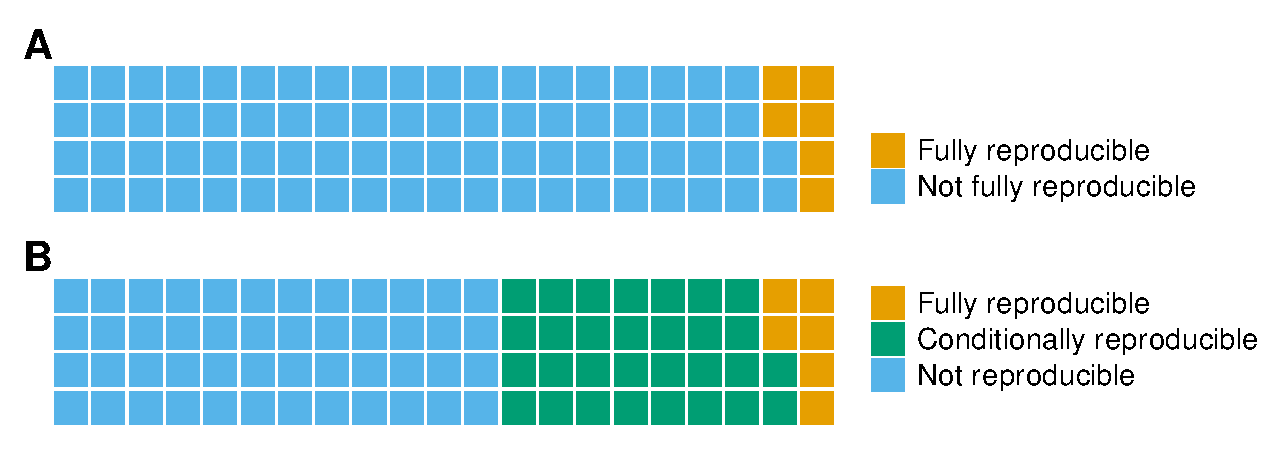
\includegraphics{../../figs/fig1} 

}

\caption{\normalfont
\textbf{(A)} Proportion of power analyses that were fully reproducible (dark purple) using the information provided in the article or supplemental materials and those that could not be reproduced (light purple) based on the provided information. \textbf{(B)} Same data as that shown in (A); however, the power analyses that were conditionally reproducible (pink) when certain assumptions were made regarding missing parameters are now highlighted. Each square represents one power analysis in the sample.}\label{fig:fig1}
\end{figure}




\clearpage

\begin{figure}

{\centering 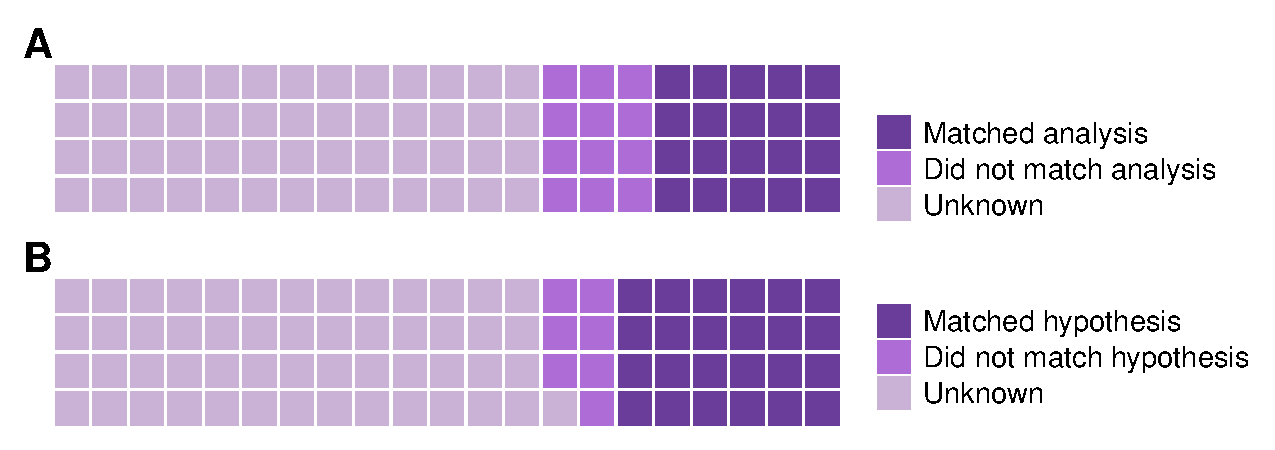
\includegraphics{../../figs/fig2} 

}

\caption{\normalfont
\textbf{(A)} Proportion of power analyses wherein the statistical test used in the power analysis matched the one used in the data analysis (dark purple), did not match (pink), or was not reported with sufficient information to determine if the analyses matched (light purple). \textbf{(B)} Proportion of power analyses that included a statistical test that addressed one of the hypotheses in the study (dark purple), included a test that did not address any hypotheses in the study (pink), or was not reported with sufficient detail to determine if the test addressed a hypothesis (light purple). Each square represents one power analysis in the sample.}\label{fig:fig2}
\end{figure}




\clearpage

\hypertarget{exploratory-analyses}{%
\subsection{Exploratory Analyses}\label{exploratory-analyses}}

Several exploratory analyses were conducted to gather more information about the current state of the reproducibility of power analyses in motor behavior research.

\hypertarget{trouble-spots}{%
\subsubsection{Trouble Spots}\label{trouble-spots}}

We noted that critical information required to reproduce power analyses was frequently missing: The statistical test and information about the effect size. We observed that 62\% (\emph{n} = 52) of the power analyses did not include the statistical test, 48\% (\emph{n} = 40) did not include the type of effect size (e.g., \emph{d}, \(f^2\), \emph{r}), and 17\% (\emph{n} = 14) did not include the value of the effect size.

\hypertarget{gpower-considerations}{%
\subsubsection{G*Power Considerations}\label{gpower-considerations}}

G*Power (Faul et al., 2009) was the chosen software in all studies that reported which software was used (74\%; \emph{n} = 62). However, in at least 7\% (\emph{n} = 6) of those studies, G*Power does not provide an accurate power calculation for the statistical design of the study. Further, although G*Power's user-friendly interface facilitates the process of conducting power analyses, the software's settings require careful use. For example, when partial eta-squared is used as the effect size in a power analysis in G*Power, but was calculated in SPSS, then failing to change the settings from default to \emph{as in SPSS} can result in considerably smaller sample sizes. We investigated the impact of this setting on sample size estimation across the 8 experiments that reported using partial eta-squared as the effect size and used G*Power with the default setting to conduct the analysis. As seen in Figure \ref{fig:fig3}B, sample size estimation increased across all experiments when the \emph{as in SPSS} setting was used, with the number of additional subjects needed ranging from 8 (Carnegie et al., 2020) to 240 (Uiga et al., 2020).

\hypertarget{rare-air}{%
\subsubsection{Rare Air}\label{rare-air}}

Ideally, power analyses should be a) fully reproducible, b) the statistical test used in the power analysis should match the test used in the data analysis and c) at least one of the hypotheses, and d) the appropriate software with e) the appropriate settings should be used to obtain an accurate sample size estimation. Only three studies (4\%; see Figure \ref{fig:fig4}) met all five of these criteria (Daou et al., 2019; Harry et al., 2019; Rhoads et al., 2019).

\clearpage

\begin{figure}

{\centering 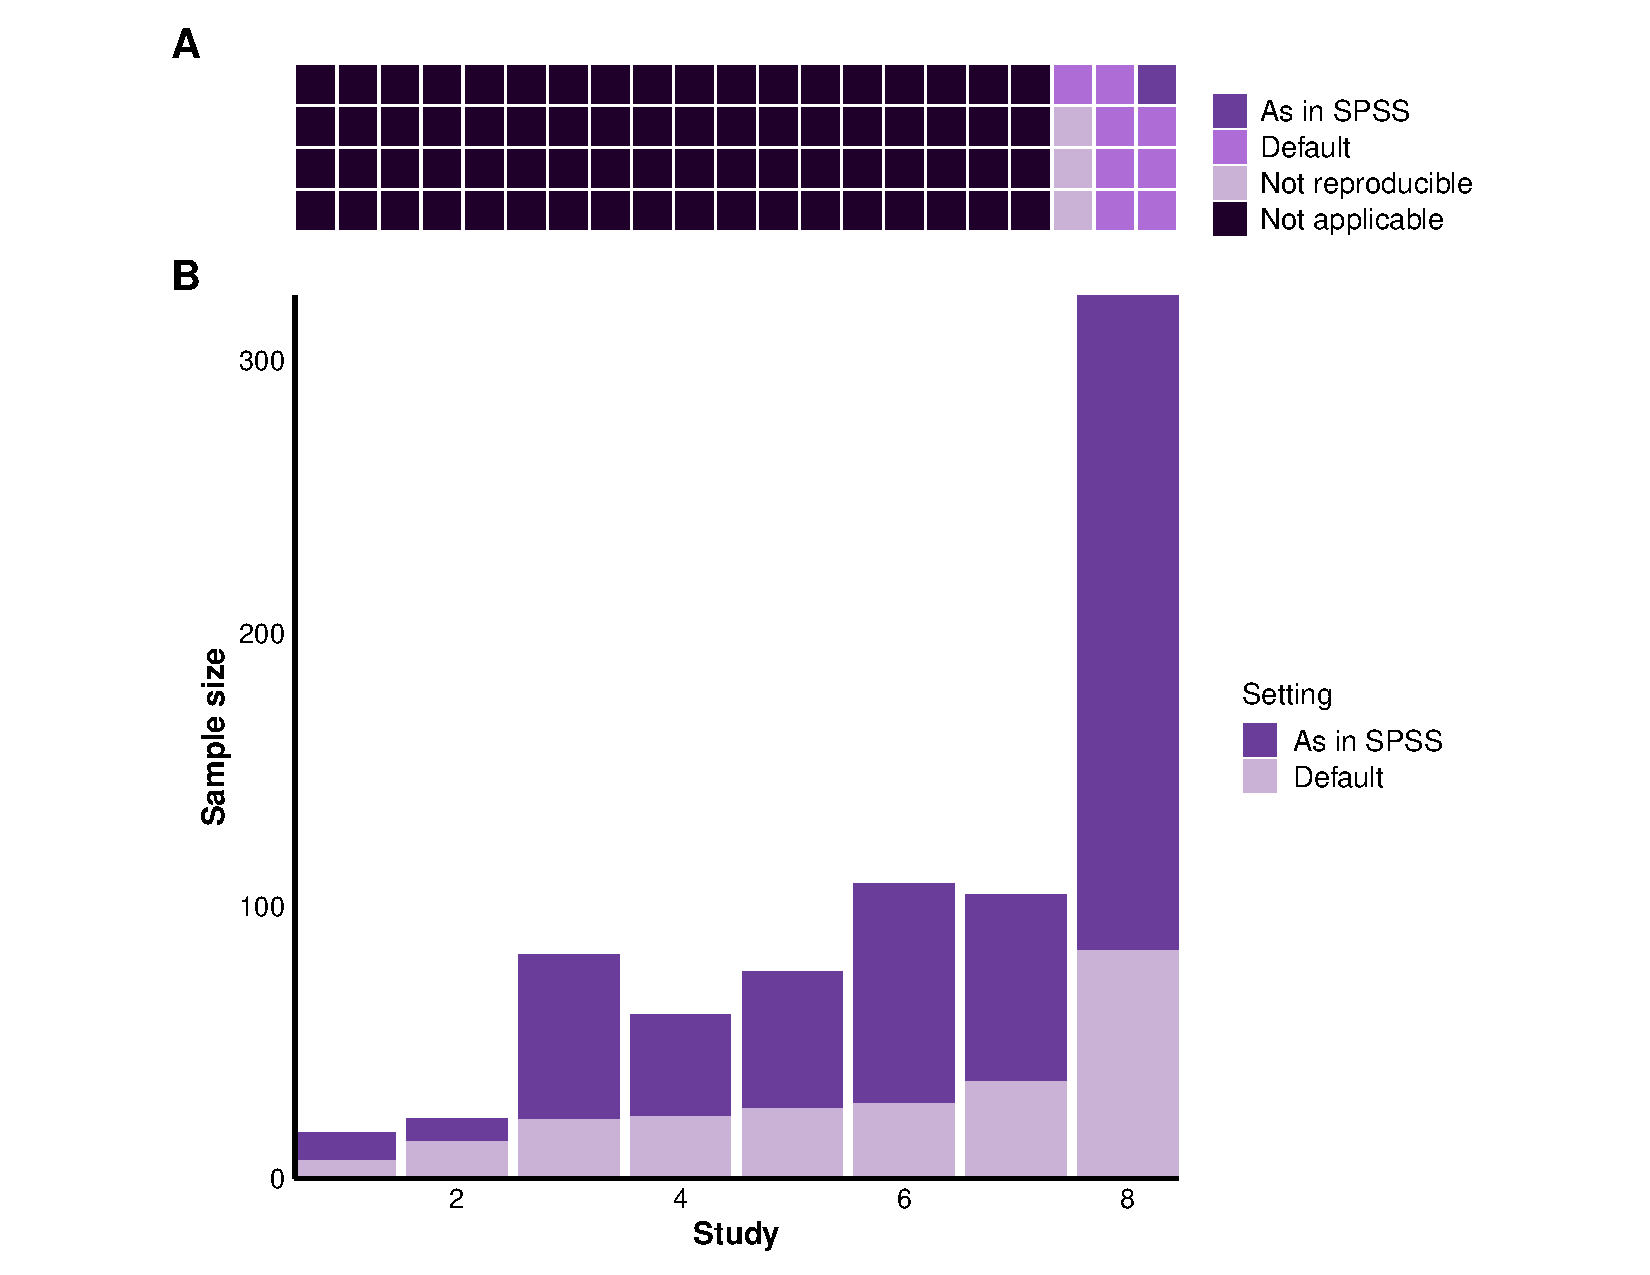
\includegraphics{../../figs/fig3} 

}

\caption{\normalfont
\textbf{(A)} Proportion of power analyses that included partial eta-squared \((\eta_{p}^2)\) as the effect size measure and used the \emph{as in SPSS} setting in G*Power (dark purple), the default setting (pink), were not reproducible (light purple), or did not include partial eta-squared as an effect size measure (black). Each square represents one power analysis in the sample. \textbf{(B)} A comparison of the required sample size based on chosen setting in G*Power when using partial eta-squared as an effect size measure. The sample size calculated by the eight studies that used the default settings and partial eta-squared as an effect size measure is shown in light purple. In contrast, if the partial eta-squared was originally calculated in SPSS, then using the appropriate \emph{as in SPSS} setting would have resulted in substantially larger sample sizes for each study, with the difference represented by the dark purple bars.}\label{fig:fig3}
\end{figure}




\clearpage

\begin{figure}

{\centering 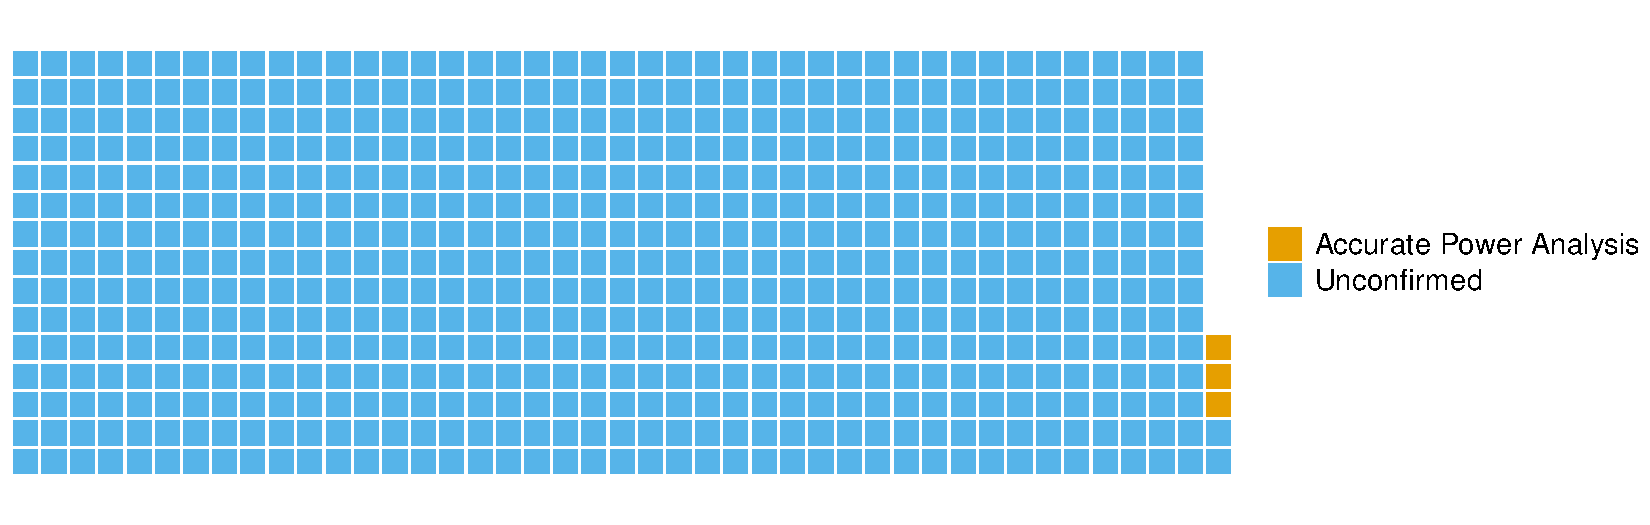
\includegraphics{../../figs/fig4} 

}

\caption{\normalfont
Proportion of accurate power analyses (dark purple). An accurate power analysis had to be 1) reproducible, 2) include a statistical test that addressed at least one hypothesis and was used in the data analysis, and 3) were conducted with the appropriate software and settings. All other studies from the full sample of articles surveyed failed to meet these criteria (light purple). Each square represents one study.}\label{fig:fig4}
\end{figure}




\clearpage

\hypertarget{discussion}{%
\section{Discussion}\label{discussion}}

\emph{A priori} power analyses are a critical tool for designing informative studies and an important step toward high quality research. Inaccurate power analyses, however, can have the opposite effect as they may lead to underpowered study designs. Detecting, and even preventing, power analysis errors depends on the ability to successfully reproduce a given analysis, which requires reporting of pertinent information. The goal of the present study was to assess the current state of power analysis reproducibility in the motor behavior domain by evaluating 84 power analyses reported in 83 research articles published in the \emph{Journal of Motor Behavior}, \emph{Human Movement Science}, and the \emph{Journal of Motor Learning and Development} between January 2019 and June 2021. Specifically, following a preregistered analysis plan, we assessed the proportion of power analyses that could be reproduced with the information reported in the article or supplementary material, the proportion of power analyses that could be reproduced conditional on making assumptions for missing parameters in the article, the proportion of studies wherein the statistical test used in the power analysis matched the test used in the data analysis, the proportion of studies wherein the statistical test used in the power analysis addressed the study's primary hypothesis, and finally, the proportion of studies that conducted a power analysis in G*Power and used the default settings when computing the effect size parameter from partial eta-squared.

We were unable to reproduce 93\% of the power analyses in the sample using only the information provided in the article or shared as supplementary information. By making assumptions for missing parameters, we were able to reproduce 43\% of the power analyses, although this of course comes with caveats. Different parameters can yield the same sample size estimation, so despite our efforts to make plausible assumptions this approach does not guarantee that the original analyses adopted the same parameters we assumed. Therefore, 43\% represents the upper bound on reproducibility with the truth likely being even more concerning. Common reasons as to why power analysis reproducibility failed include lack of information regarding the design used in the power analysis, the type of effect size, and the effect size value. A missing effect size value is particularly problematic because one cannot simply guess what effect size authors are targeting.

The process of conducting power analyses is facilitated by an abundance of user-friendly and openly available programs, including G*Power (Faul et al., 2009), which is commonly used in social and behavioral research. In our sample, all studies (\emph{n} = 62) that reported the software used G*Power, establishing a preference for this program in the motor behavior domain. While conducting a power analysis in G*Power can be straightforward, easy-to-make mistakes when using the software can lead to inaccurate power calculations. For instance, G*Power is not suitable for calculating power for mixed factorial designs with three or more within-subject factors, which require the use of other packages such as Superpower (Lakens \& Caldwell, 2021). In our sample, at least 7\% of the power analyses adopted designs that are too complex for G*Power. More critically, G*Power's method to compute the effect size partial eta-squared differs from the method used in SPSS. If researchers are basing their effect size target on previous estimates of partial eta-squared, and those estimates were calculated in SPSS, they need to change the effect size specification under \emph{Options} from \emph{default} to \emph{as in SPSS} (G*Power version: 3.1.9.7). Across the power analyses assessed in the present study, 10 used partial eta-squared as the effect size parameter in G*Power but only one used the \emph{as in SPSS} setting. All 8 experiments that originally used the default setting would have been underpowered to detect the effect of interest if it was originally calculated in SPSS.

A lack of thoroughly reported and vetted power analyses contributes to the proliferation of underpowered studies, which combined with selection for significant results threatens the credibility of our literature. The impact of low power and selection bias is well illustrated by the growing body of metascience calling into question the reliability of research paradigms long considered robust (Carter et al., 2015; e.g., Maier et al., 2022; Vohs et al., 2021), such as self-controlled practice in the motor learning domain (McKay et al., in-press). In a recent meta-analysis, McKay and colleagues estimated the benefit to motor learning of giving learners control over an aspect of their environment is trivially small, if existent, after correcting for publication bias. Nevertheless, the average effect size in the published literature was \emph{g} = .54, suggesting apparent benefits. Similarly, another meta-analysis (McKay, Bacelar, et al., 2022) investigated the second motivational factor in OPTIMAL theory (Wulf \& Lewthwaite, 2016), enhanced expectancies. The analysis found that despite an average benefit of \emph{g} = .54 in the published literature, the true effect of enhanced expectancies is likely much smaller, if it exists at all. The studies examined in these meta-analyses had median sample sizes of \emph{n} = 14 and \emph{n} = 18, requiring effects larger than \emph{g} = .8 to achieve significance with an independent \emph{t}-test. Therefore, selectively publishing significant results in these literatures meant publishing an abundance of large effects, making it possible for even null effects to appear moderately beneficial on average.

It is not only the extant but the future literature that is affected by underpowered studies. Small studies with positive results generate inflated effect sizes (Gelman \& Carlin, 2014) and when these inflated effect sizes are used in power calculations for future studies, those studies become underpowered as well. This snowball effect can lead to uncertainty, research waste, and overall issues with replication as additional studies that are unlikely to be informative continue to be conducted and discarded, or reported when positive (Open Science Collaboration, 2015).

We have reviewed evidence that power analyses have been reported infrequently in the motor behavior literature (McKay, Corson, et al., 2022). When power analyses were reported, they were rarely reproducible without making assumptions, and even then, most power analyses could not be reproduced. Meanwhile, there is growing evidence that the average power among motor behavior studies is low, making the literature vulnerable to more severe bias from various selective reporting mechanisms (McKay, Hussien, et al., 2022; McKay et al., in-press; e.g., Mesquida et al., 2022). Here, we argue that power analyses can easily be reported in a reproducible fashion and doing so is a progressive step toward improved research quality overall. Thus, in the next section, we present several recommendations to facilitate power analysis reproducibility in the future.

\hypertarget{power-analysis-reproducibility-recommendations-for-future-studies}{%
\subsection{Power Analysis Reproducibility: Recommendations for Future Studies}\label{power-analysis-reproducibility-recommendations-for-future-studies}}

Two simple practices can ensure power analysis reproducibility: complete reporting and sharing of code. The minimum parameters required to reproduce a power analysis are the type of effect size and its value (e.g., \emph{d}, \(f^2\), \emph{r}), the accepted false-positive rate (i.e., alpha), the target power value (e.g., 80\%), the specific statistical test, and the required sample size. Several additional parameters may be required to reproduce a specific analysis. A helpful strategy for G*Power users is to report every possible input variable. Although one can technically reproduce a power analysis without knowing the primary hypothesis, we argue that researchers should also explicitly state their main hypothesis so others (e.g., collaborators, peer-reviewers, and readers) can assess whether a given study was powered to detect the main effect of interest.

A common trouble spot among studies in our sample was the description of the statistical test. We suggest making use of standardized language in power analysis software. This is a straightforward approach that offers researchers a clear way to describe the power analysis components, which is not only helpful from a practical standpoint, but it also reduces uncertainty. For instance, if a researcher reports the use of a test from the ANOVA family in G*Power, five different options are possible. However, if she reports the use of the statistical test \emph{ANOVA: Repeated measures, within-between interaction}, only one option is available. Reporting the exact language used in the software will clarify the statistical test for readers.

\begingroup\fontsize{10}{12}\selectfont

\begin{landscape}
\begin{longtable}[l]{ll}
\caption{\label{tab:table1}Recommendations for ensuring reproducible power analyses}\\
\toprule
Recommendation & Examples\\
\midrule
Report all necessary parameters & Effect size type and value: d = .40\\
\addlinespace
 & Accepted false positive rate: alpha = .05\\
\addlinespace
 & One or two-tailed test: Two-tailed\\
\addlinespace
 & Target power: 80\%; Alternatively, accepted false negative rate: beta = .20\\
\addlinespace
 & Specific statistical test: t-test - difference between two independent means (two groups).\\
\addlinespace
 & Required sample size: 200\\
\addlinespace
 & Primary hypothesis: We predict group A to have higher scores on the DV than group B.\\
\addlinespace
 & \\
\addlinespace
Share the code & G*Power: Protocol of power analyses tab -> Save -> Share\\
\addlinespace
 & Anything in R: Save the script -> Share\\
\bottomrule
\end{longtable}
\end{landscape}
\endgroup{}

The second simple practice that will ensure power analysis reproducibility is sharing the code. It is easy to save the exact protocol used in the power analysis in software such as G*Power, Superpower, and \texttt{R}. In G*Power, the \emph{Protocol of power analyses} tab includes all the details of the power analysis and can be saved as a PDF. Researchers can make this file available online in a repository such as the Open Science Framework (\url{https://osf.io}) or as part of supplementary material. Sharing code is a great strategy for ensuring the reproducibility of power analyses and primary analyses alike.

The benefits of adopting the practices we have presented go beyond power analysis reproducibility. For one, these practices increase research transparency, a key goal of the Open Science movement. Clear reporting can also assist other researchers in determining parameters for their own power analyses, which is especially helpful for researchers conducting their first power analysis for a given hypothesis. Although power analyses are best used for study planning, they can be conducted at any time. Therefore, the most informative power analyses are not just reproducible, but preregistered. Fortunately, another benefit of completing a reproducible power analysis while planning a study is that it represents a huge step toward preregistration. The study's primary hypothesis, smallest effect size of interest, statistical test to answer the research question, desired error rates, and the intended sample size comprise at least 50\% of a preregistration form (e.g., \url{https://aspredicted.org} form, see supplementary material). To illustrate the potential symbiotic relationship between reproducible power analysis reporting and preregistration, in our sample, 50\% of the experiments considered fully reproducible had a preregistered analysis plan, while only 0.47\% of the overall sample was preregistered.

\hypertarget{limitations}{%
\subsection{Limitations}\label{limitations}}

Since we were unable to reproduce most of the power analyses, we cannot assess whether the primary deficit among studies is in power analysis quality or in reporting quality. Further, when power analyses were reproducible, we made no effort to evaluate the quality of the evidence produced by those studies. Although we are optimistic that increased adoption of reproducible power analyses will benefit the quality of research in our field, we recognize that power analyses are not a panacea for bias in research. Indeed, while we recommend powering studies to detect the smallest effect size of interest, we give no guidance on how to select this value. This is no small challenge for researchers and future metascience should focus on developing methods for choosing which effects are likely to be important in each study. \textcolor{blue}{In the meantime, it is important for researchers to think carefully about the specific effects they are investigating and not rely on effect size benchmarks to inform their power analyses. In fact, the benchmarks recommended by Cohen} (1988) \textcolor{blue}{and used in G\*Power change depending on the type of analysis, rendering them inconsistent and illogical for use in sample size planning} (Correll et al., 2020). \textcolor{blue}{Instead, researchers should think about raw differences they would not want to miss to help arrive at a smallest effect of interest.}

\hypertarget{conclusion}{%
\section{Conclusion}\label{conclusion}}

From a sample of 635 motor behavior studies, 84 included a power analysis, and of those we found three that were both appropriate and reproducible. There is converging evidence that motor behavior research tends to be underpowered, perhaps because power analyses are not yet being leveraged to ensure a study produces informative results. Researchers can improve this situation by comprehensively reporting the details of their power analyses and sharing their code. Journals can improve this situation by asking for reproducible power analyses as a condition of publication. Finally, peer reviewers can improve this situation by double-checking that the power analysis reported in a submission can be reproduced and has been appropriately conducted. Together, the sports science community can improve the quality of our research with relatively simple adjustments to the research workflow.

\vspace{5ex}

\hypertarget{author-contributions-credit-taxonomy}{%
\subsection{Author Contributions (CRediT Taxonomy)}\label{author-contributions-credit-taxonomy}}

\noindent Conceptualization: BM, MFBB, MJC

\noindent Data curation: BM, MJC

\noindent Formal analysis: BM, MFBB

\noindent Funding acquisition: MJC

\noindent Investigation: BM, MFBB

\noindent Methodology: BM, MFBB

\noindent Project administration: BM, MJC

\noindent Software: BM, MJC

\noindent Supervision: MJC

\noindent Validation: BM, MJC

\noindent Visualization: BM, MJC

\noindent Writing -- original draft: BM, MFBB, MJC

\noindent Writing -- review \& editing: BM, MFBB, MJC

\hypertarget{open-science-practices}{%
\subsection{Open Science Practices}\label{open-science-practices}}

\noindent The preregistration, data, and code for this study can be accessed using either of these links: \url{https://github.com/cartermaclab/proj_power-reproducibility-motor-behaviour} or \url{https://osf.io/9a6m8/}. \textcolor{blue}{An unrefereed version of this paper can be found at https://doi.org/10.51224/SRXIV.184}

\hypertarget{conflicts-of-interest}{%
\subsection{Conflicts of Interest}\label{conflicts-of-interest}}

\noindent All authors declare no conflicts of interest.

\hypertarget{funding}{%
\subsection{Funding}\label{funding}}

\noindent This work was supported by the Natural Sciences and Engineering Research Council (NSERC) of Canada (RGPIN-2018-05589; MJC) and McMaster University (MJC).

\pagebreak

\hypertarget{references}{%
\section{References}\label{references}}

\vspace{2ex}

\hypertarget{refs}{}
\begin{CSLReferences}{1}{0}
\leavevmode\vadjust pre{\hypertarget{ref-Abt2020}{}}%
Abt, G., Boreham, C., Davison, G., Jackson, R., Nevill, A., Wallace, E., \& Williams, M. (2020). Power, precision, and sample size estimation in sport and exercise science research. \emph{Journal of Sports Sciences}, \emph{38}(17), 1933--1935. \url{https://doi.org/10.1080/02640414.2020.1776002}

\leavevmode\vadjust pre{\hypertarget{ref-R-papaja}{}}%
Aust, F., \& Barth, M. (2020). \emph{{papaja}: {Prepare} reproducible {APA} journal articles with {R Markdown}}. \url{https://github.com/crsh/papaja}

\leavevmode\vadjust pre{\hypertarget{ref-Bacelar2022}{}}%
Bacelar, M. F. B., Parma, J. O., Murrah, W. M., \& Miller, M. W. (2022). Meta-analyzing enhanced expectancies on motor learning: Positive effects but methodological concerns. \emph{International Review of Sport and Exercise Psychology}, \emph{0}(0), 1--30. \url{https://doi.org/10.1080/1750984X.2022.2042839}

\leavevmode\vadjust pre{\hypertarget{ref-Borg2022}{}}%
Borg, D. N., Barnett, A., Caldwell, A. R., White, N., \& Stewart, I. (2022). \emph{The bias for statistical significance in sport and exercise medicine}. \url{https://doi.org/10.31219/osf.io/t7yfc}

\leavevmode\vadjust pre{\hypertarget{ref-Carnegie2020}{}}%
Carnegie, E., Marchant, D., Towers, S., \& Ellison, P. (2020). Beyond visual fixations and gaze behaviour. Using pupillometry to examine the mechanisms in the planning and motor performance of a golf putt. \emph{Human Movement Science}, \emph{71}, 102622. \url{https://doi.org/10.1016/j.humov.2020.102622}

\leavevmode\vadjust pre{\hypertarget{ref-Carter2015}{}}%
Carter, E. C., Kofler, L. M., Forster, D. E., \& McCullough, M. E. (2015). A series of meta-analytic tests of the depletion effect: Self-control does not seem to rely on a limited resource. \emph{Journal of Experimental Psychology: General}, \emph{144}(4), 796--815. \url{https://doi.org/10.1037/xge0000083}

\leavevmode\vadjust pre{\hypertarget{ref-R-extrafont}{}}%
Chang, W. (2022). \emph{Extrafont: Tools for using fonts}. \url{https://CRAN.R-project.org/package=extrafont}

\leavevmode\vadjust pre{\hypertarget{ref-Cohen1988}{}}%
Cohen, J. (1988). \emph{Statistical power analysis for the behavioral sciences} (2nd ed.). Routledge.

\leavevmode\vadjust pre{\hypertarget{ref-correll2020}{}}%
Correll, J., Mellinger, C., McClelland, G. H., \& Judd, C. M. (2020). Avoid {Cohen}'s {``{Small},''} {``{Medium},''} and {``{Large}''} for {Power} {Analysis}. \emph{Trends in Cognitive Sciences}, \emph{24}(3), 200--207. \url{https://doi.org/10.1016/j.tics.2019.12.009}

\leavevmode\vadjust pre{\hypertarget{ref-Daou2019}{}}%
Daou, M., Rhoads, J. A., Jacobs, T., Lohse, K. R., \& Miller, M. W. (2019). Does limiting pre-movement time during practice eliminate the benefit of practicing while expecting to teach? \emph{Human Movement Science}, \emph{64}, 153--163. \url{https://doi.org/10.1016/j.humov.2018.11.017}

\leavevmode\vadjust pre{\hypertarget{ref-debruine2021}{}}%
DeBruine, L., Krystalli, A., \& Heiss, A. (2021). \emph{Faux: {Simulation} for {Factorial} {Designs}}. \url{https://CRAN.R-project.org/package=faux}

\leavevmode\vadjust pre{\hypertarget{ref-Faul2009}{}}%
Faul, F., Erdfelder, E., Buchner, A., \& Lang, A.-G. (2009). Statistical power analyses using g*power 3.1: Tests for correlation and regression analyses. \emph{Behavior Research Methods}, \emph{41}(4), 1149--1160. \url{https://doi.org/10.3758/BRM.41.4.1149}

\leavevmode\vadjust pre{\hypertarget{ref-R-daff}{}}%
Fitzpatrick, P., de Jonge, E., \& Warnes, G. R. (2019). \emph{Daff: Diff, patch and merge for data.frames}. \url{https://CRAN.R-project.org/package=daff}

\leavevmode\vadjust pre{\hypertarget{ref-Gelman2014}{}}%
Gelman, A., \& Carlin, J. (2014). Beyond power calculations: Assessing type s (sign) and type m (magnitude) errors. \emph{Perspectives on Psychological Science}, \emph{9}(6), 641--651.

\leavevmode\vadjust pre{\hypertarget{ref-Harry2019}{}}%
Harry, J. R., Lanier, R., Nunley, B., \& Blinch, J. (2019). Focus of attention effects on lower extremity biomechanics during vertical jump landings. \emph{Human Movement Science}, \emph{68}, 102521. \url{https://doi.org/10.1016/j.humov.2019.102521}

\leavevmode\vadjust pre{\hypertarget{ref-Lakens2021a}{}}%
Lakens, D. (2021). \emph{Sample size justification}.

\leavevmode\vadjust pre{\hypertarget{ref-Lakens2021b}{}}%
Lakens, D., \& Caldwell, A. R. (2021). Simulation-based power analysis for factorial analysis of variance designs. \emph{Advances in Methods and Practices in Psychological Science}, \emph{4}(1), 2515245920951503. \url{https://doi.org/10.1177/2515245920951503}

\leavevmode\vadjust pre{\hypertarget{ref-Lohse2016}{}}%
Lohse, K., Buchanan, T., \& Miller, M. (2016). Underpowered and overworked: Problems with data analysis in motor learning studies. \emph{Journal of Motor Learning and Development}, \emph{4}(1), 37--58. \url{https://doi.org/10.1123/jmld.2015-0010}

\leavevmode\vadjust pre{\hypertarget{ref-Maier2022}{}}%
Maier, M., Bartoš, F., Stanley, T. D., Shanks, D. R., Harris, A. J. L., \& Wagenmakers, E.-J. (2022). No evidence for nudging after adjusting for publication bias. \emph{Proceedings of the National Academy of Sciences}, \emph{119}(31), e2200300119. \url{https://doi.org/10.1073/pnas.2200300119}

\leavevmode\vadjust pre{\hypertarget{ref-McCrum2022}{}}%
McCrum, C., Beek, J. van, Schumacher, C., Janssen, S., \& Van Hooren, B. (2022). Sample size justifications in gait \& posture. \emph{Gait \& Posture}, \emph{92}, 333--337. \url{https://doi.org/10.1016/j.gaitpost.2021.12.010}

\leavevmode\vadjust pre{\hypertarget{ref-McKay2022c}{}}%
McKay, B., Bacelar, M., Parma, J. O., Miller, M. W., \& Carter, M. J. (2022). \emph{The combination of reporting bias and underpowered study designs have substantially exaggerated the motor learning benefits of self-controlled practice and enhanced expectancies: A meta-analysis}. PsyArXiv. \url{https://doi.org/10.31234/osf.io/3nhtc}

\leavevmode\vadjust pre{\hypertarget{ref-McKay2022b}{}}%
McKay, B., Corson, A., Vinh, M.-A., Jeyarajan, G., Tandon, C., Brooks, H., Hubley, J., \& Carter, M. J. (2022). \emph{Low prevalence of a priori power analyses in motor behavior research}. SportRxiv. \url{https://sportrxiv.org/index.php/server/preprint/view/175}

\leavevmode\vadjust pre{\hypertarget{ref-McKay2022a}{}}%
McKay, B., Hussien, J., Vinh, M.-A., Mir-Orefice, A., Brooks, H., \& Ste-Marie, D. M. (2022). Meta-analysis of the reduced relative feedback frequency effect on motor learning and performance. \emph{Psychology of Sport and Exercise}, 102165. \url{https://doi.org/10.1016/j.psychsport.2022.102165}

\leavevmode\vadjust pre{\hypertarget{ref-McKay2021}{}}%
McKay, B., Yantha, Z. D., Hussien, J., Carter, M. J., \& Ste-Marie, D. M. (in-press). Meta-analytic findings in the self-controlled motor learning literature: Underpowered, biased, and lacking evidential value. \emph{Meta-Psychology}. \url{https://doi.org/10.31234/osf.io/8d3nb}

\leavevmode\vadjust pre{\hypertarget{ref-Mesquida2022}{}}%
Mesquida, C., Murphy, J., Lakens, D., \& Warne, J. (2022). \emph{Replication concerns in sports science: A narrative review of selected methodological issues in the field}. SportRxiv. \url{https://sportrxiv.org/index.php/server/preprint/view/127}

\leavevmode\vadjust pre{\hypertarget{ref-OSC2015}{}}%
Open Science Collaboration. (2015). Estimating the reproducibility of psychological science. \emph{Science}, \emph{349}(6251), aac4716. \url{https://doi.org/10.1126/science.aac4716}

\leavevmode\vadjust pre{\hypertarget{ref-qiu2021}{}}%
Qiu, W. (2021). \emph{{powerMediation}: {Power}/{Sample} {Size} {Calculation} for {Mediation} {Analysis}}. \url{https://CRAN.R-project.org/package=powerMediation}

\leavevmode\vadjust pre{\hypertarget{ref-R-base}{}}%
R Core Team. (2021). \emph{R: A language and environment for statistical computing}. R Foundation for Statistical Computing. \url{https://www.R-project.org/}

\leavevmode\vadjust pre{\hypertarget{ref-Rhoads2019}{}}%
Rhoads, J. A., Daou, M., Lohse, K. R., \& Miller, M. W. (2019). The effects of expecting to teach and actually teaching on motor learning. \emph{Journal of Motor Learning \& Development}, \emph{7}(1), 84--105.

\leavevmode\vadjust pre{\hypertarget{ref-Robinson2021}{}}%
Robinson, M. A., Vanrenterghem, J., \& Pataky, T. C. (2021). Sample size estimation for biomechanical waveforms: Current practice, recommendations and a comparison to discrete power analysis. \emph{Journal of Biomechanics}, \emph{122}, 110451. \url{https://doi.org/10.1016/j.jbiomech.2021.110451}

\leavevmode\vadjust pre{\hypertarget{ref-R-waffle}{}}%
Rudis, B., \& Gandy, D. (2019). \emph{Waffle: Create waffle chart visualizations}. \url{https://gitlab.com/hrbrmstr/waffle}

\leavevmode\vadjust pre{\hypertarget{ref-Twomey2021}{}}%
Twomey, R., Yingling, V., Warne, J., Schneider, C., McCrum, C., Atkins, W., Murphy, J., Medina, C. R., Harlley, S., \& Caldwell, A. (2021). The nature of our literature: A registered report on the positive result rate and reporting practices in kinesiology. \emph{Communications in Kinesiology}, \emph{1}(3). \url{https://doi.org/10.51224/cik.v1i3.43}

\leavevmode\vadjust pre{\hypertarget{ref-Uiga2020}{}}%
Uiga, L., Poolton, J. M., Capio, C. M., Wilson, M. R., Ryu, D., \& Masters, R. S. W. (2020). The role of conscious processing of movements during balance by young and older adults. \emph{Human Movement Science}, \emph{70}, 102566. \url{https://doi.org/10.1016/j.humov.2019.102566}

\leavevmode\vadjust pre{\hypertarget{ref-R-renv}{}}%
Ushey, K. (2022). \emph{Renv: Project environments}. \url{https://CRAN.R-project.org/package=renv}

\leavevmode\vadjust pre{\hypertarget{ref-Vohs2021}{}}%
Vohs, K., Schmeichel, B., Lohmann, S., Gronau, Q. F., Finley, A. J., Wagenmakers, E.-J., \& Albarracín, D. (2021). \emph{A multi-site preregistered paradigmatic test of the ego depletion effect}.

\leavevmode\vadjust pre{\hypertarget{ref-Westfall2015}{}}%
Westfall, J. (2015). PANGEA: Power analysis for general ANOVA designs. \emph{Unpublished Manuscript. Available at Http://Jakewestfall. Org/Publications/Pangea. Pdf}, \emph{4}.

\leavevmode\vadjust pre{\hypertarget{ref-R-tidyverse}{}}%
Wickham, H., Averick, M., Bryan, J., Chang, W., McGowan, L. D., François, R., Grolemund, G., Hayes, A., Henry, L., Hester, J., Kuhn, M., Pedersen, T. L., Miller, E., Bache, S. M., Müller, K., Ooms, J., Robinson, D., Seidel, D. P., Spinu, V., \ldots{} Yutani, H. (2019). Welcome to the {tidyverse}. \emph{Journal of Open Source Software}, \emph{4}(43), 1686. \url{https://doi.org/10.21105/joss.01686}

\leavevmode\vadjust pre{\hypertarget{ref-Wulf2016}{}}%
Wulf, G., \& Lewthwaite, R. (2016). Optimizing performance through intrinsic motivation and attention for learning: The OPTIMAL theory of motor learning. \emph{Psychonomic Bulletin \& Review}, \emph{23}(5), 1382--1414.

\end{CSLReferences}


\end{document}
